% Ubah judul dan label berikut sesuai dengan yang diinginkan.

% % Ubah paragraf-paragraf pada bagian ini sesuai dengan yang diinginkan.

% % Contoh input beberapa gambar pada halaman.
% \begin{figure*}
%   \centering
%   \subfloat[Hasil A]{\includegraphics[width=.4\textwidth]{example-image-a}
%     \label{fig:hasila}}
%   \hfil
%   \subfloat[Hasil B]{\includegraphics[width=.4\textwidth]{example-image-b}
%     \label{fig:hasilb}}
%   \caption{Contoh input beberapa gambar.}
%   \label{fig:hasil}
% \end{figure*}

% \lipsum[16-18]

% % Contoh input potongan kode dari file.
% \lstinputlisting[
%   language=Python,
%   caption={Program perhitungan bilangan prima.},
%   label={lst:bilanganprima}
% ]{program/bilangan-prima.py}

% \lipsum[19-20]

% Update the title and label below as desired.
\section{Results and Discussion}
\label{sec:resultsanddiscussion}

% Update the paragraphs in this section as desired.

% % Example of inserting multiple images on a page.
% \begin{figure*}
%     \centering
%     \subfloat[Result A]{\includegraphics[width=.4\textwidth]{example-image-a}
%         \label{fig:resulta}}
%     \hfil
%     \subfloat[Result B]{\includegraphics[width=.4\textwidth]{example-image-b}
%         \label{fig:resultb}}
%     \caption{Example of inserting multiple images.}
%     \label{fig:result}
% \end{figure*}

% \lipsum[16-18]

% % Example of including a code snippet from a file.
% \lstinputlisting[
%     language=Python,
%     caption={Prime number calculation program.},
%     label={lst:primenumbers}
% ]{program/prime-numbers.py}

% \lipsum[19-20]

\subsection{Model Form Testing}
\label{sec:modelanalysis}
The model form tested is based on the model form explained in Subsection \ref{subsec:poseclassification}. This test was conducted to observe the impact of the LSTM model structure on the classification performance of sign language movements. The differences in the layers used are as follows:

\begin{table}[H]
    \caption{LSTM Model Structure}
    \label{tb:modelsummary}
    \centering
    \begin{tabular}{ll}
      \hline
      \textbf{Model} & \textbf{Layer Structure} \\
      \hline
      Model 1 & 
      \begin{tabular}[t]{l}
        \emph{LSTM} 1 (128 units, \emph{relu}) \\
        \emph{Dropout} 1 (0.5) \\
        \emph{LSTM} 2 (64 units, \emph{relu}) \\
        \emph{Dropout} 2 (0.5) \\
      \end{tabular} \\
      \hline
      Model 2 & 
      \begin{tabular}[t]{l}
        \emph{TimeDistributed} (\emph{Dense}, 128 units, \emph{tanh}) \\
        \emph{LSTM} 1 (64 units, \emph{tanh}) \\
        \emph{Dropout} 1 (0.5) \\
      \end{tabular} \\
      \hline
      Model 3 & 
      \begin{tabular}[t]{l}
        \emph{TimeDistributed} (\emph{Dense}, 128 units, \emph{tanh}) \\
        \emph{LSTM} 1 (128 units, \emph{tanh}) \\
        \emph{Dropout} 1 (0.5) \\
        \emph{LSTM} 2 (64 units, \emph{tanh}) \\
        \emph{Dropout} 2 (0.5) \\
      \end{tabular} \\
      \hline
    \end{tabular}
  \end{table}
  
The model is trained with 12 epochs and a dataset partition of 70:30, with 70\% training data and 30\% validation data. The trained model is then tested based on the existing test data and provides the following classification results:

\begin{table}[H]
    \caption{LSTM Model Evaluation Results}
    \label{tb:modelevaluation}
    \centering
    \begin{tabular}{lllll}
      \hline
      \textbf{Model} & \textbf{\emph{Avg. Accuracy}} & \textbf{\emph{Avg. Precision}} & \textbf{\emph{Avg. Recall}} & \textbf{\emph{Avg. F1-Score}} \\
      \hline
      Model 1 & 0.85 & 0.85 & 0.85 & 0.83 \\
      Model 2 & 0.93 & 0.95 & 0.94 & 0.94 \\
      Model 3 & 0.99 & 0.99 & 0.98 & 0.99 \\
      \hline
    \end{tabular}
  \end{table}
  
Based on Table \ref{tb:modelevaluation}, it can be seen that there is a relationship between the increased complexity of the LSTM model and the classification performance of sign language movements. This can be observed in that the third model produces the best performance with the use of a TimeDistributed layer and 2 LSTM layers.

\subsection{Light Condition Testing}
\label{sec:lightanalysis}

This test will observe the model's ability to adapt to changes in room light intensity. This test is performed using the third model tested in Table \ref{tb:modelsummary}, with the user standing 300 cm away from the camera. Light intensity data was collected using the Lux Meter application.

\begin{table}[H]
  \caption{Light Level Evaluation Results}
  \label{tb:lightevaluation}
  \centering
  \begin{tabular}{llll}
    \hline
    \textbf{Light} & \textbf{Accuracy} & \emph{\textbf{Avg. Processing Time}} & \emph{\textbf{Avg. Complete Time}} \\
    \hline
    35 lux & 0.89 & 0.0938 & 3.0335 \\
    80 lux & 0.96 & 0.0918 & 2.9928 \\
    125 lux & 1.00 & 0.0923 & 2.4777 \\
    \hline
  \end{tabular}
\end{table}

Based on Table \ref{tb:lightevaluation}, it can be seen that a reduction in light intensity in a room causes an increase in processing time and complete time. However, in terms of accuracy, the 125 lux light intensity has the best accuracy compared to other light intensities. This can be due to the camera's ability to capture the user's sign movements more clearly.

\subsection{Distance Condition Testing}
\label{sec:distanceanalysis}

This test will observe the model's ability to adapt to changes in the distance between the user and the camera. This test is performed using the third model tested in Table \ref{tb:modelsummary}, with a light intensity of 125 lux. Note that the user's sign movements should be clearly visible on the camera.

\begin{table}[H]
  \caption{Distance Evaluation Results}
  \label{tb:distanceevaluation}
  \centering
  \begin{tabular}{llll}
    \hline
    \textbf{Distance} & \textbf{Accuracy} & \emph{\textbf{Avg. Processing Time}} & \emph{\textbf{Avg. Complete Time}} \\
    \hline
    180 cm & 0.89 & 0.1017 & 2.3660 \\
    240 cm & 0.96 & 0.0994 & 2.5098 \\
    300 cm & 1.00 & 0.0997 & 2.7918 \\
    \hline
  \end{tabular}
\end{table}

Based on Table \ref{tb:distanceevaluation}, it can be seen that increasing the distance results in better model classification accuracy. This is due to the camera clearly capturing the user's sign movements as the distance increases. However, increasing the distance results in an increase in complete time, while processing time tends to be fluctuating.

\subsection{Different Subject Testing}
\label{sec:subjectanalysis}

This test is conducted to observe the model's ability to adapt to changes in subjects other than the user. This test is performed using the third model tested in Table \ref{tb:modelevaluation}, with a light intensity of 125 lux and a camera distance of 300 cm. The subjects who participated in this test can be seen in Table \ref{tb:subjectconditions}.

\begin{table}[H]
  \caption{Different Subject Variations}
  \label{tb:subjectconditions}
  \centering
  \begin{tabular}{ll}
    \hline
    \textbf{Gender} & \textbf{Subject Image} \\
    \hline
    Female & 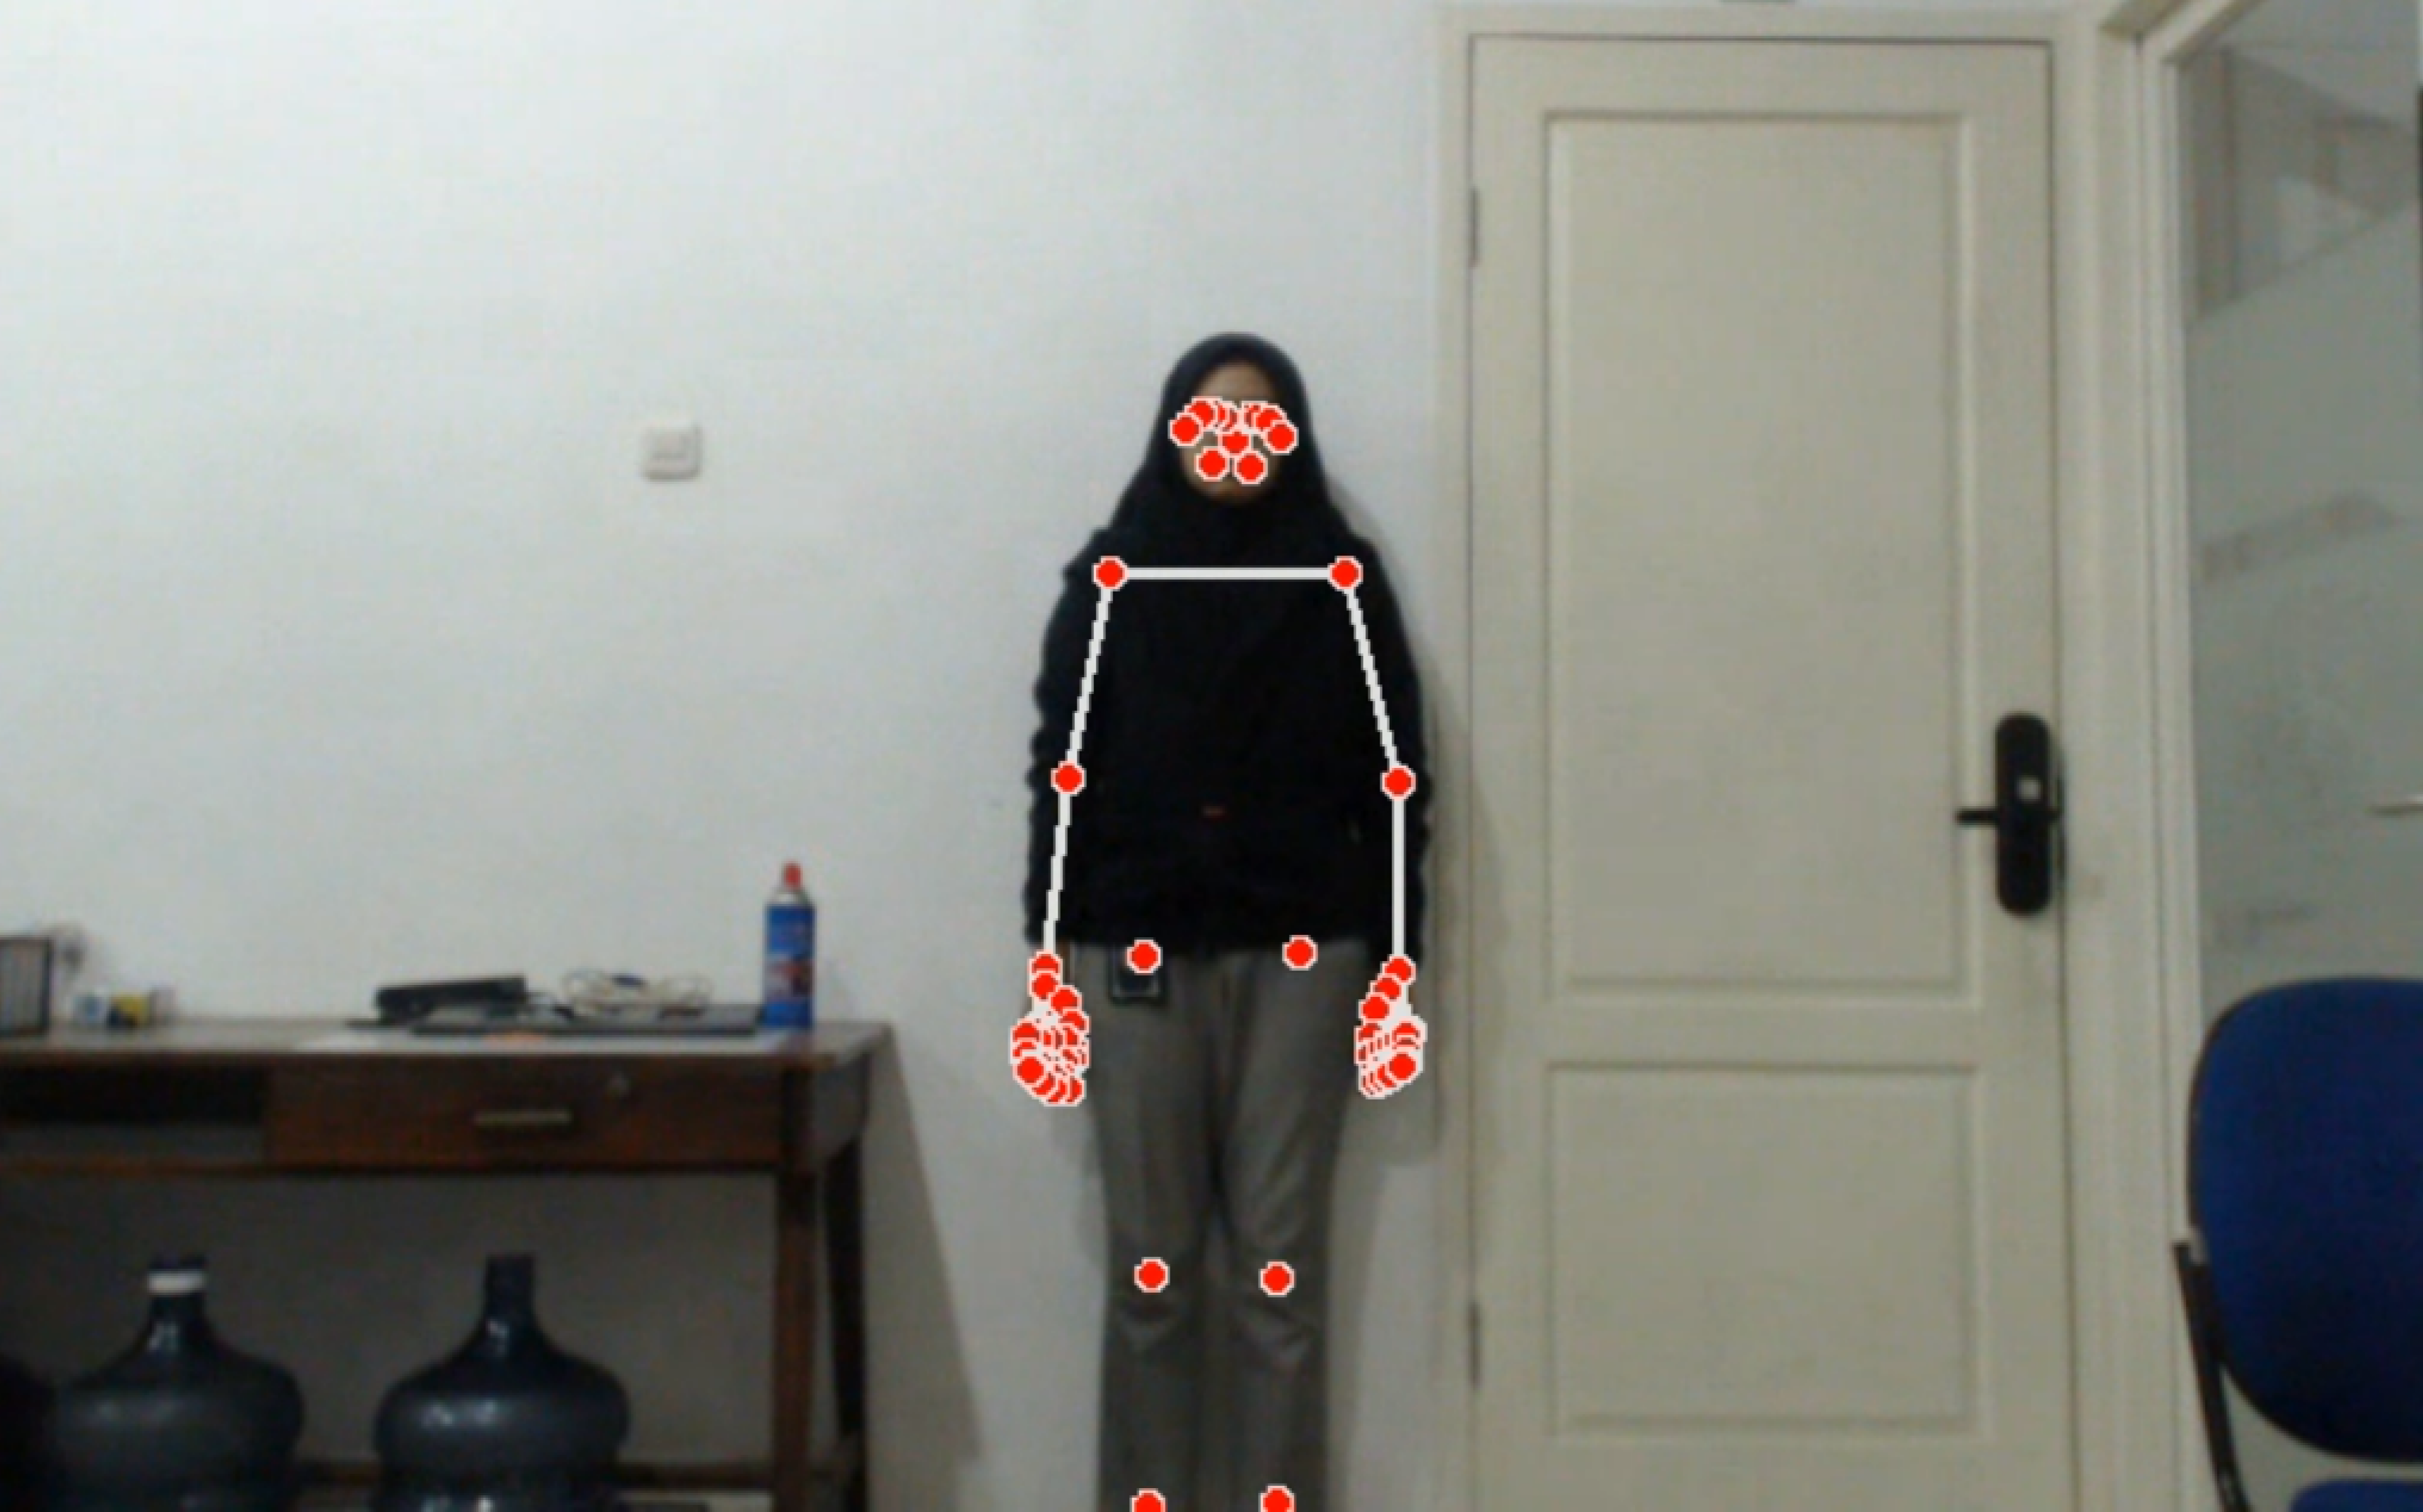
\includegraphics[scale=0.12]{gambar/bab4-rani.png} \\
    \hline
    Male & 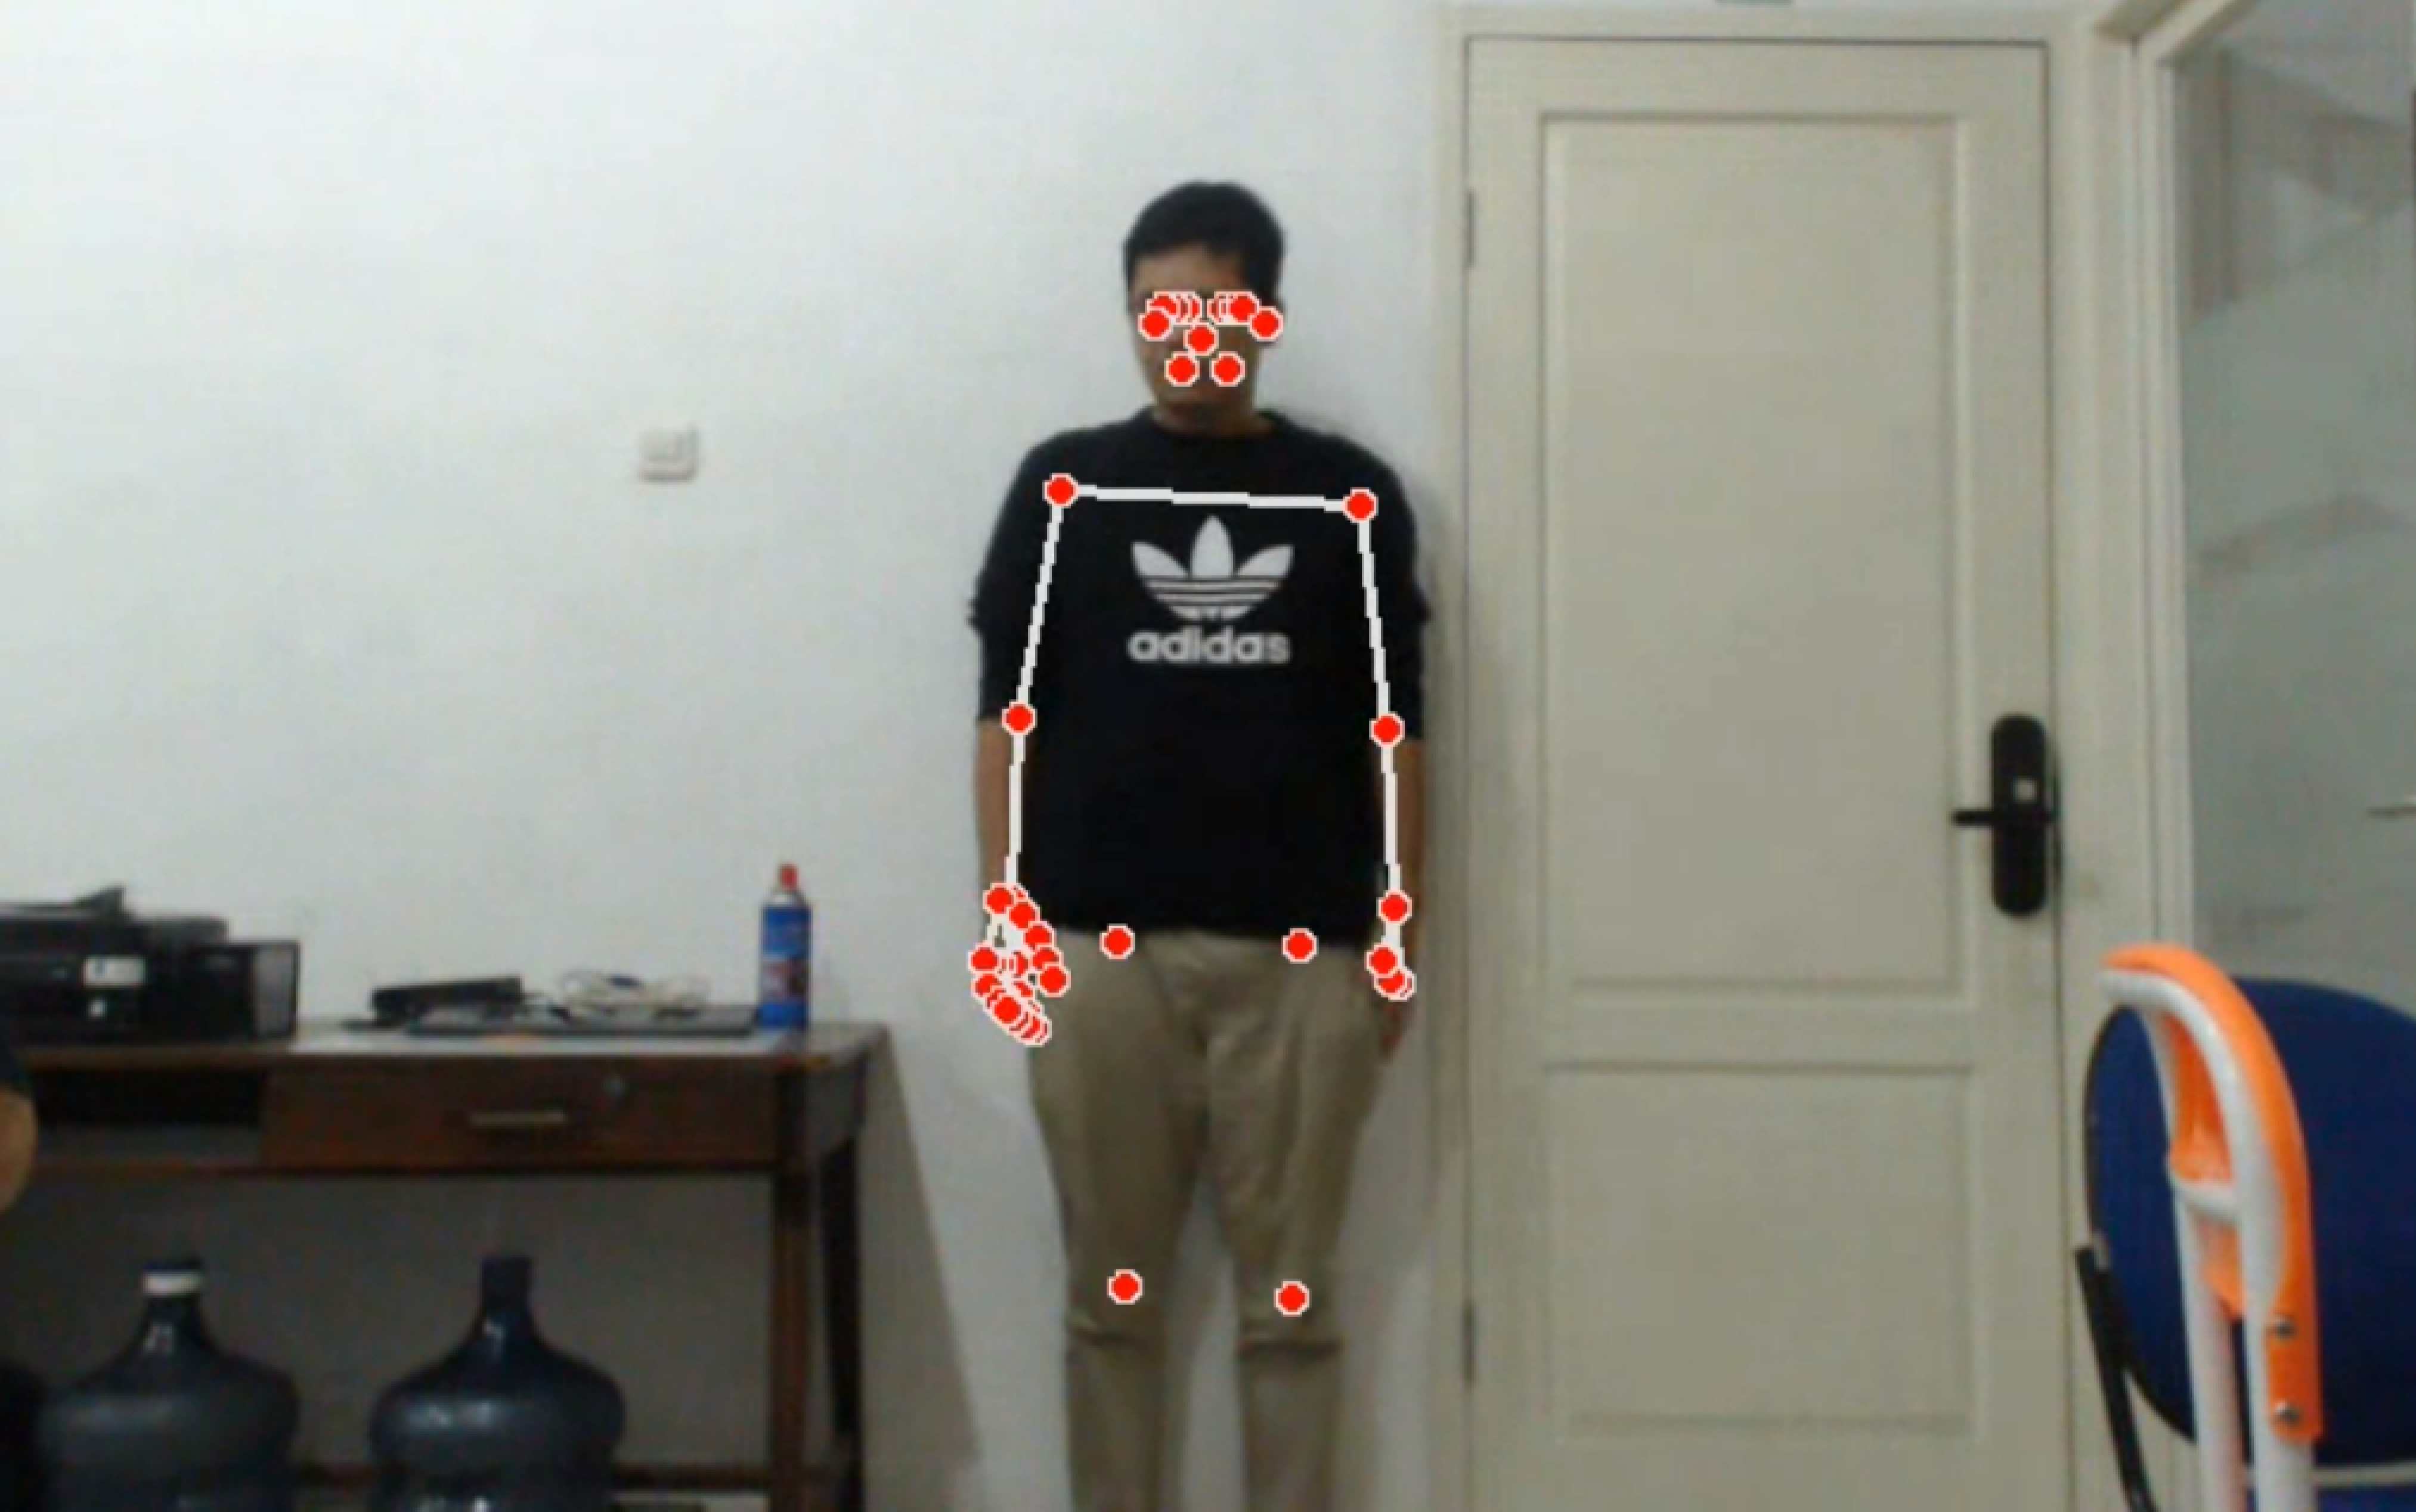
\includegraphics[scale=0.12]{gambar/bab4-evan.png} \\
    \hline
  \end{tabular}
\end{table}

\begin{table}[H]
  \caption{Different Subject Evaluation Results}
  \label{tb:subjectevaluation}
  \centering
  \begin{tabular}{llll}
    \hline
    \textbf{Subject} & \textbf{Accuracy} & \emph{\textbf{Avg. Processing Time}} & \emph{\textbf{Avg. Complete Time}} \\
    \hline
    Female & 0.93 & 0.0988 & 2.6636 \\
    Male & 0.93 & 0.0973 & 2.8191 \\
    \hline
  \end{tabular}
\end{table}

Based on Table \ref{tb:subjectevaluation}, it can be seen that the model can classify different subjects. Data normalization has resulted in a scale-invariant and position-invariant model. The model classification accuracy shows a very good value of 0.93 or 93\%. The average processing time and complete time also show values that are not much different from the previous tests, with the average processing time ranging around 0.098 and the complete time around 2.74.

\subsection{Sentence Formation and Voice Conversion Testing}
\label{sec:sentenceanalysis}

This test is conducted to understand how the translation system is used to form a series of sentences and perform voice conversion based on the formed sentences. The sentence formation in this system refers to Subsection \ref{subsec:controlsystem}. The sentences will be formed based on a combination of detected vocabulary. The full combination of vocabulary is in Table \ref{tb:vocabularycombination}. This test is performed using the third model tested in Table \ref{tb:modelevaluation}, with a light intensity of 125 lux and a camera distance of 300 cm. A maximum of three repetitions is done for each vocabulary. For each vocabulary combination, control vocabulary is also tested, including "standby," "delete," and "translate."

\begin{table}[H]
  \caption{Vocabulary and Sentence Combinations}
  \label{tb:vocabularycombination}
  \centering
  \begin{tabular}{ll}
    \hline
    \textbf{Vocabulary Combinations} & \textbf{Sentences} \\
    \hline
    "Maaf" + "Siapa" + "Nama" & "Maaf siapa nama kamu?" \\
    "Maaf" + "Tolong" + "Saya" & "Maaf tolong bantu saya" \\
    "Maaf" + "Rumah" + "Siapa" & "Maaf ini rumah siapa?" \\
    "Rumah" + "Saya" & "Ini rumah saya" \\
    "Rumah" + "Siapa" & "Ini rumah siapa?" \\
    "Siapa" + "Nama" & "Siapa nama kamu?" \\
    "Tolong" + "Saya" & "Tolong bantu saya" \\
    \hline
  \end{tabular}
\end{table}

\begin{table}[H]
  \caption{Vocabulary Combination Evaluation Results}
  \label{tb:combinationevaluation}
  \centering
  \begin{tabular}{llll}
    \hline
    \textbf{Combinations} & \textbf{Accuracy} & \emph{\textbf{Avg. Processing Time}} & \emph{\textbf{Avg. Complete Time}} \\
    \hline
    2  & 1.00 & 0.0993 & 2.8303 \\
    3  & 0.93 & 0.0981 & 2.0513 \\
    \hline
  \end{tabular}
\end{table}

As seen in Table \ref{tb:combinationevaluation}, the model has successfully formed sentences by combining them sequentially and continuously. This is shown by the accuracy of sentences formed from the combination of 2 vocabularies being 1.00 and the combination of 3 vocabularies being 0.93. The average processing time and average complete time values did not change significantly compared to the tests carried out continuously. In forming the sentence "Ini rumah saya", there was a classification error in the sign movement "home", which was classified as "delete." This is due to the high similarity between the sign movements "rumah" and "delete." Overall, the system's success rate in forming sentences is 0.857 or 85.7\%.

Overall, the tests show that the system has good performance in translating sign movements in relatively large numbers and in real-time.

\begin{figure}[ht]
    \centering
    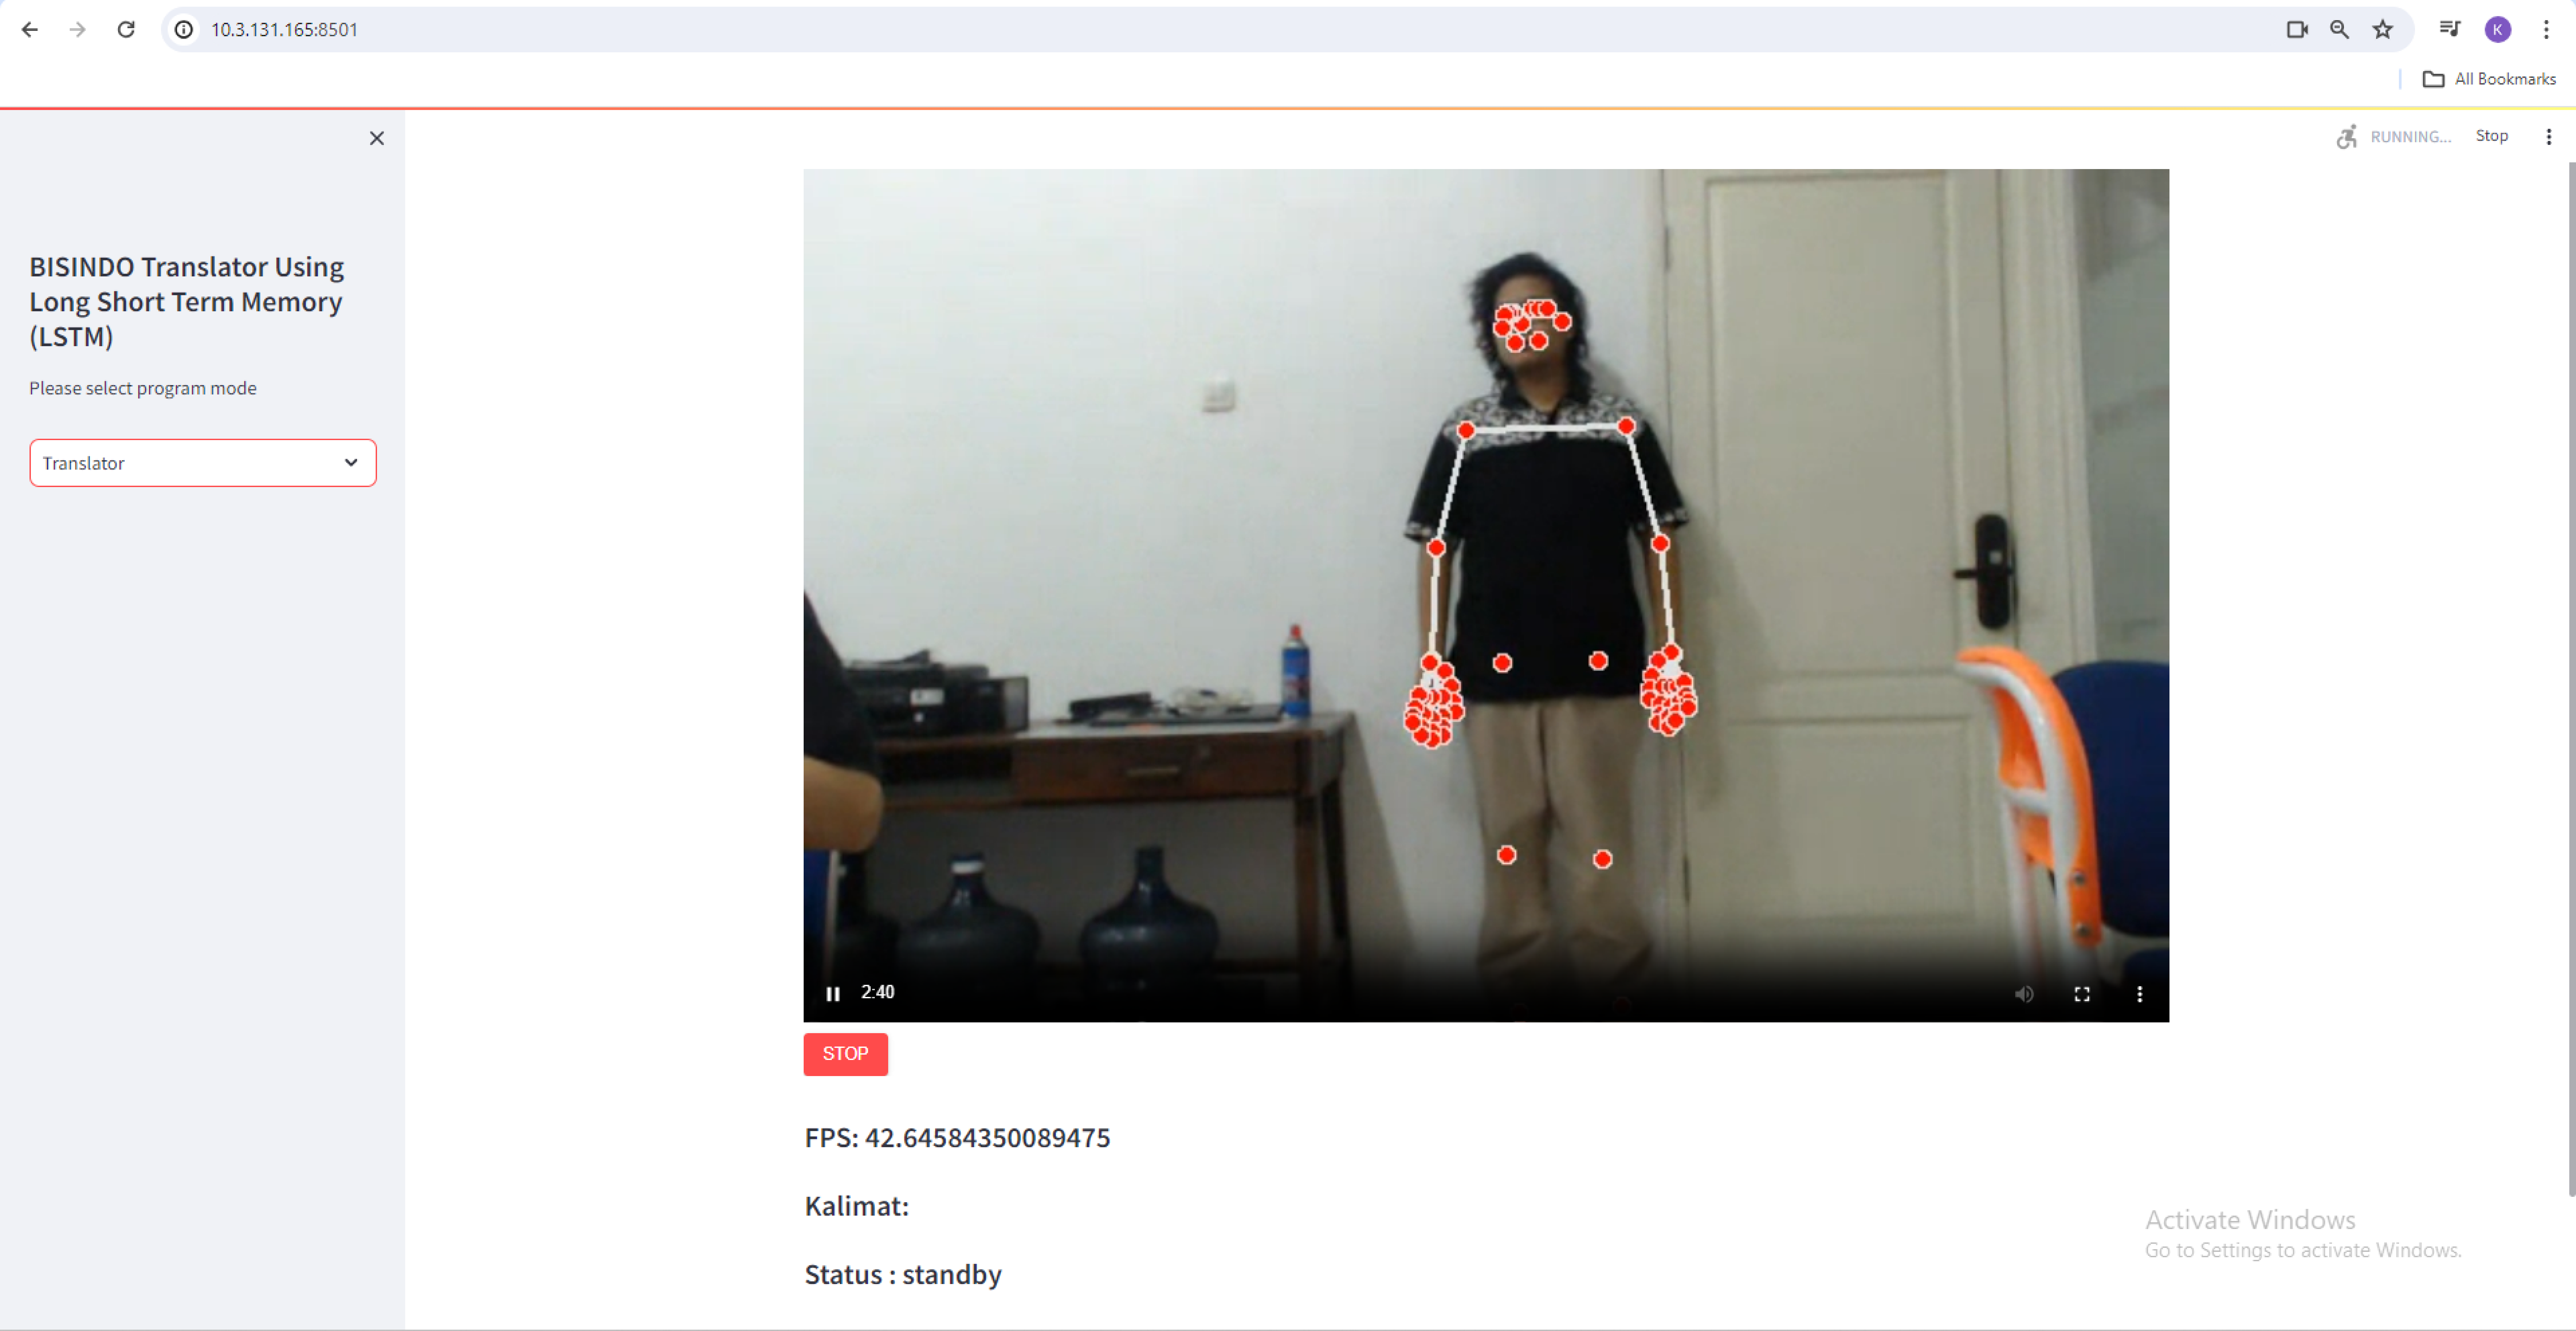
\includegraphics[scale=0.12]{gambar/bab3-layoutweb.png}
    \caption{System Testing Results}
    \label{fig:layoutweb}
\end{figure}
